\documentclass{article}
\usepackage[utf8]{inputenc}
\usepackage[english, ukrainian]{babel}
\usepackage{fontsize}
\usepackage{geometry}
\usepackage{amsthm}
\usepackage{amsfonts}
\usepackage{graphicx}
\usepackage[ruled]{algorithm2e}
\usepackage{hyperref}
\usepackage{biblatex}
\usepackage{csquotes}
\usepackage{mathtools}
\usepackage{amsmath}
\usepackage{amssymb}
\usepackage{bbm}
\usepackage{tabularx}
\usepackage{xcolor}

\usepackage{tikz}
\usetikzlibrary{decorations.pathmorphing}

\usepackage{enumitem}
\usepackage{nicefrac}

\usepackage{listings}
\definecolor{codegreen}{rgb}{0,0.6,0}
\definecolor{codegray}{rgb}{0.5,0.5,0.5}
\definecolor{codepurple}{rgb}{0.58,0,0.82}
\definecolor{backcolour}{rgb}{0.95,0.95,0.92}

\lstdefinestyle{mystyle}{
    backgroundcolor=\color{backcolour},   
    commentstyle=\color{codegreen},
    keywordstyle=\color{magenta},
    numberstyle=\tiny\color{codegray},
    stringstyle=\color{codepurple},
    basicstyle=\ttfamily\footnotesize,
    breakatwhitespace=false,         
    breaklines=true,                 
    captionpos=b,                    
    keepspaces=true,                 
    numbers=left,                    
    numbersep=5pt,                  
    showspaces=false,                
    showstringspaces=false,
    showtabs=false,                  
    tabsize=2
}

\lstset{style=mystyle}
\hypersetup{colorlinks=true, linkcolor=[RGB]{255, 3, 209}, citecolor={black}}
\graphicspath{ {../Images/} }

\begin{document}
    \begin{titlepage}
        \begin{center}
            \begin{center}
                НАЦІОНАЛЬНИЙ ТЕХНІЧНИЙ УНІВЕРСИТЕТ УКРАЇНИ
                «КИЇВСЬКИЙ ПОЛІТЕХНІЧНИЙ ІНСТИТУТ імені Ігоря СІКОРСЬКОГО»

                Фізико-технічний інститут
            \end{center}
        $\newline$
        \vspace{3.3cm}
        
        {КОМП’ЮТЕРНИЙ ПРАКТИКУМ № 6.\\РОЗВ’ЯЗАННЯ ЗАДАЧІ КОШІ МЕТОДАМИ РУНГЕ-КУТТА ТА АДАМСА}
        \vspace{5cm}
        \begin{flushright}
            Виконав\\студент 3 курсу ФТІ\\групи ФІ-21\\Климентьєв Максим Андрійович
            
            \vspace{1cm}

            Перевірив:\\\underline{\hspace{5cm}}\\Оцінка:\\\underline{\hspace{5cm}}
        \end{flushright}
        \vspace{3cm}
        Київ --- 2025
        \end{center}
    \end{titlepage}
    \newpage

    \pagenumbering{gobble}
    \tableofcontents
    \cleardoublepage
    \pagenumbering{arabic}
    \setcounter{page}{3}

    \newpage
    \section{Завдання}
    Методами Рунге-Кутта та Адамса-Башфорта четвертого порядку розв'язати задачу Коші. На
    початку інтервалу у необхідній кількості точок значення для методу Адамса визначити методом
    Рунге-Кутта четвертого порядку.

    \section{Вимоги до звіту}
    Для деякого фіксованого h потрібно навести:
    \begin{itemize}
        \item значення точної функції розв’язку y(x);
        \item значення наближеного розв'язку y(x) у тих самих точках, одержані обома методами;
        \item значення функції помилки e(x) для обох методів (порівняти із «теоретичною» точністю);
    \end{itemize}
    У звіті наводять:
    \begin{itemize}
        \item графіки точного розв'язку та обох наближених - на одному рисунку;
        \item графіки обох помилок - на другому рисунку;
        \item лістинг програми.
    \end{itemize}

    \section{ПОСТАНОВКА ЗАДАЧІ}
        Рівняння має вигляд:
        $y' = (1 - y) \cdot x^2 + F(x)$
        Покласти $h = 0.1$. Початкові умови $x(0)$ визначити, використовуючи точне значення розв’язку.

        Нехай розв’язок відомий та визначається згідно з варіантами:

        Необхідно підставити розв’язок у рівняння та визначити F(x) у правій частині. Таким
        чином, відомим є вигляд рівняння та його точний розв’язок, за допомогою числових методів далі
        будуємо наближений розв’язок.

    \section{Вихідна система}
        \begin{tabular}{ |c|c| }
            \hline
            Варіант & Точний розв’язок \\ 
            \hline
            10 & $y = x \cdot \sin(x)$\\ 
            \hline
        \end{tabular}

    \newpage
    \section{Таблиця результатів}
        \begin{table}[h!]
            \centering
            \begin{tabular}{|c|c|c|c|c|c|}
                \hline
                $x$ & 0.0 & 0.1 & 0.2 & 0.3 & 0.4 \\
                \hline
                $y_{true}$ & 0.0 & 0.00998 & 0.03973 & 0.08866 & 0.15577 \\
                \hline
                $y_{runge}$ & 0.0 & 0.00998 & 0.03973 & 0.08866 & 0.15577 \\
                \hline
                $y_{adam}$ & 0.0 & 0.00998 & 0.03973 & 0.08866 & 0.15576 \\
                \hline
            \end{tabular}
            \caption{Порівняння рішень на відрізку $[0.0, 0.4]$}
        \end{table}

        \begin{table}[h!]
            \centering
            \begin{tabular}{|c|c|c|c|c|c|}
                \hline
                $x$ & 0.5 & 0.6 & 0.7 & 0.8 & 0.9 \\
                \hline
                $y_{true}$ & 0.23971 & 0.33879 & 0.45095 & 0.57388 & 0.70499 \\
                \hline
                $y_{runge}$ & 0.23971 & 0.33879 & 0.45095 & 0.57388 & 0.70499 \\
                \hline
                $y_{adam}$ & 0.2397 & 0.33877 & 0.45093 & 0.57385 & 0.70495 \\
                \hline
            \end{tabular}
            \caption{Порівняння рішень на відрізку $[0.5, 0.9]$}
        \end{table}

        \begin{table}[h!]
            \centering
            \begin{tabular}{|c|c|c|c|c|c|}
                \hline
                $x$ & 1.0 & 1.1 & 1.2 & 1.3 & 1.4 \\
                \hline
                $y_{true}$ & 0.84147 & 0.98033 & 1.11845 & 1.25263 & 1.37963 \\
                \hline
                $y_{runge}$ & 0.84147 & 0.98033 & 1.11845 & 1.25262 & 1.37963 \\
                \hline
                $y_{adam}$ & 0.84142 & 0.98026 & 1.11837 & 1.25255 & 1.37955 \\
                \hline
            \end{tabular}
            \caption{Порівняння рішень на відрізку $[1.0, 1.4]$}
        \end{table}

        \begin{table}[h!]
            \centering
            \begin{tabular}{|c|c|c|c|c|c|}
                \hline
                $x$ & 1.5 & 1.6 & 1.7 & 1.8 & 1.9 \\
                \hline
                $y_{true}$ & 1.49624 & 1.59932 & 1.68583 & 1.75293 & 1.79797 \\
                \hline
                $y_{runge}$ & 1.49624 & 1.59931 & 1.68582 & 1.75291 & 1.79794 \\
                \hline
                $y_{adam}$ & 1.49616 & 1.59924 & 1.68575 & 1.75285 & 1.79791 \\
                \hline
            \end{tabular}
            \caption{Порівняння рішень на відрізку $[1.5, 1.9]$}
        \end{table}

        \begin{table}[h!]
            \centering
            \begin{tabular}{|c|c|c|c|c|c|}
                \hline
                $x$ & 2.0 & 2.1 & 2.2 & 2.3 & 2.4 \\
                \hline
                $y_{true}$ & 1.81859 & 1.81274 & 1.77869 & 1.71512 & 1.62111 \\
                \hline
                $y_{runge}$ & 1.81856 & 1.81269 & 1.77862 & 1.71503 & 1.62099 \\
                \hline
                $y_{adam}$ & 1.81854 & 1.81269 & 1.77865 & 1.71509 & 1.62108 \\
                \hline
            \end{tabular}
            \caption{Порівняння рішень на відрізку $[2.0, 2.4]$}
        \end{table}

        \begin{table}[h!]
            \centering
            \begin{tabular}{|c|c|c|c|c|c|}
                \hline
                $x$ & 2.5 & 2.6 & 2.7 & 2.8 & 2.9 \\
                \hline
                $y_{true}$ & 1.49618 & 1.3403 & 1.15393 & 0.93797 & 0.69382 \\
                \hline
                $y_{runge}$ & 1.49603 & 1.34013 & 1.15371 & 0.93772 & 0.69354 \\
                \hline
                $y_{adam}$ & 1.49616 & 1.34029 & 1.15392 & 0.93796 & 0.69382 \\
                \hline
            \end{tabular}
            \caption{Порівняння рішень на відрізку $[2.5, 2.9]$}
        \end{table}

        \begin{table}[h!]
            \centering
            \begin{tabular}{|c|c|c|c|c|c|}
                \hline
                $x$ & 3.0 & 3.1 & 3.2 & 3.3 & 3.4 \\
                \hline
                $y_{true}$ & 0.42336 & 0.1289 & -0.1868 & -0.52056 & -0.86884 \\
                \hline
                $y_{runge}$ & 0.42305 & 0.12857 & -0.18714 & -0.5209 & -0.86916 \\
                \hline
                $y_{adam}$ & 0.42336 & 0.1289 & -0.18679 & -0.52055 & -0.86883 \\
                \hline
            \end{tabular}
            \caption{Порівняння рішень на відрізку $[3.0, 3.4]$}
        \end{table}

        \begin{table}[h!]
            \centering
            \begin{tabular}{|c|c|c|c|c|c|}
                \hline
                $x$ & 3.5 & 3.6 & 3.7 & 3.8 & 3.9 \\
                \hline
                $y_{true}$ & -1.22774 & -1.59307 & -1.96039 & -2.32506 & -2.68229 \\
                \hline
                $y_{runge}$ & -1.22801 & -1.59326 & -1.96045 & -2.32493 & -2.68192 \\
                \hline
                $y_{adam}$ & -1.22773 & -1.59306 & -1.96038 & -2.32505 & -2.68227 \\
                \hline
            \end{tabular}
            \caption{Порівняння рішень на відрізку $[3.5, 3.9]$}
        \end{table}

        \begin{table}[h!]
            \centering
            \begin{tabular}{|c|c|c|c|c|c|}
                \hline
                $x$ & 4.0 & 4.1 & 4.2 & 4.3 & 4.4 \\
                \hline
                $y_{true}$ & -3.02721 & -3.35494 & -3.66062 & -3.93951 & -4.18705 \\
                \hline
                $y_{runge}$ & -3.02652 & -3.35383 & -3.65898 & -3.93721 & -4.18392 \\
                \hline
                $y_{adam}$ & -3.0272 & -3.3549 & -3.66069 & -3.93915 & -4.18857 \\
                \hline
            \end{tabular}
            \caption{Порівняння рішень на відрізку $[4.0, 4.4]$}
        \end{table}

    \newpage
    \section{Графіки}
        \begin{figure}[h!]
            \centering
            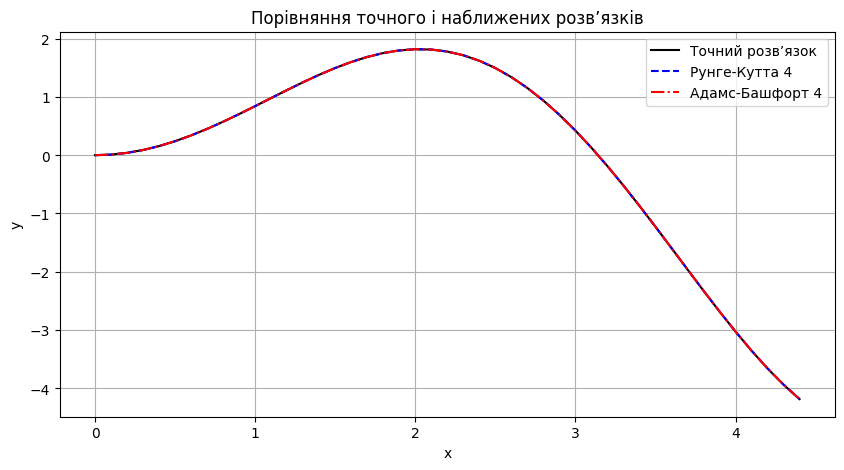
\includegraphics[scale=0.5]{compare.png}
            \caption{Графік точного та наближених розв’язків}
        \end{figure}

        \begin{figure}[h!]
            \centering
            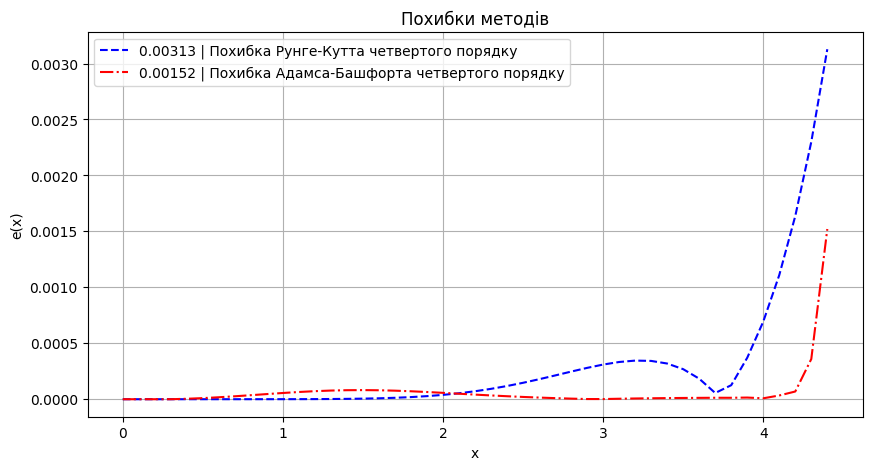
\includegraphics[scale=0.5]{error.png}
            \caption{Графік похибок методів Рунге-Кутта четвертого порядку і Адамса-Башфорта четвертого порядку}
        \end{figure}

    \newpage
    \section{Лістинг програми}
    \begin{lstlisting}[language=Python, caption=Code]
def f(x):
    return x * np.sin(x)
def f_s(x, y):
    # y'(x) = sin(x) + x cos(x)
    # sin(x) + x cos(x) = (1 - x * sin(x)) * x**2 + F(x)
    # F(x) = sin(x) + x * cos(x) - (1 - x * sin(x)) * x**2
    Fx = np.sin(x) + x * np.cos(x) - (1 - x * np.sin(x)) * x**2
    return (1 - y)*x**2 + Fx
def runge_kutta_4(x0, y0, h, n, f_s):
    x = np.zeros(n)
    y = np.zeros(n)
    x[0] = x0
    y[0] = y0
    for i in range(n-1):
        x_i = x[i]
        y_i = y[i]

        k1 = h * f_s(x_i, y_i)
        k2 = h * f_s(x_i + h/2, y_i + 1/2*k1)
        k3 = h * f_s(x_i + h/2, y_i + 1/2*k2)
        k4 = h * f_s(x_i + h, y_i + k3)

        x[i+1] = x_i + h
        y[i+1] = y_i + (k1 + 2*k2 + 2*k3 + k4)/6
    return x, y
def adams_bashforth_4(x_init, y_init, h, n, f_s):
    x = x_init.copy()
    y = np.zeros_like(y_init)
    y[:4] = y_init[:4]
    for i in range(3, n-1):
        f_n   = f_s(x[i],   y[i])
        f_n1  = f_s(x[i-1], y[i-1])
        f_n2  = f_s(x[i-2], y[i-2])
        f_n3  = f_s(x[i-3], y[i-3])

        y[i+1] = y[i] + h*(55*f_n - 59*f_n1 + 37*f_n2 - 9*f_n3)/24
    return x, y
    \end{lstlisting}
\end{document}